\documentclass[english,notitlepage, reprint]{revtex4-1}  % defines the basic parameters of the document
%For preview: skriv i terminal: latexmk -pdf -pvc filnavn



% if you want a single-column, remove reprint

% allows special characters (including æøå)
\usepackage[utf8]{inputenc}
%\usepackage[english]{babel}

%% note that you may need to download some of these packages manually, it depends on your setup.
%% I recommend downloading TeXMaker, because it includes a large library of the most common packages.

\usepackage{physics,amssymb}  % mathematical symbols (physics imports amsmath)
\include{amsmath}
\usepackage{graphicx}         % include graphics such as plots
\usepackage{xcolor}           % set colors
\usepackage{hyperref}         % automagic cross-referencing (this is GODLIKE)
\usepackage{listings}         % display code
\usepackage{subfigure}        % imports a lot of cool and useful figure commands
\usepackage{float}
%\usepackage[section]{placeins}
\usepackage{algorithm}
\usepackage[noend]{algpseudocode}
\usepackage{subfigure}
\usepackage{tikz}
\usetikzlibrary{quantikz}
% defines the color of hyperref objects
% Blending two colors:  blue!80!black  =  80% blue and 20% black
\hypersetup{ % this is just my personal choice, feel free to change things
	colorlinks,
	linkcolor={red!50!black},
	citecolor={blue!50!black},
	urlcolor={blue!80!black}}

%% Defines the style of the programming listing
%% This is actually my personal template, go ahead and change stuff if you want



%% USEFUL LINKS:
%%
%%   UiO LaTeX guides:        https://www.mn.uio.no/ifi/tjenester/it/hjelp/latex/
%%   mathematics:             https://en.wikibooks.org/wiki/LaTeX/Mathematics

%%   PHYSICS !                https://mirror.hmc.edu/ctan/macros/latex/contrib/physics/physics.pdf

%%   the basics of Tikz:       https://en.wikibooks.org/wiki/LaTeX/PGF/Tikz
%%   all the colors!:          https://en.wikibooks.org/wiki/LaTeX/Colors
%%   how to draw tables:       https://en.wikibooks.org/wiki/LaTeX/Tables
%%   code listing styles:      https://en.wikibooks.org/wiki/LaTeX/Source_Code_Listings
%%   \includegraphics          https://en.wikibooks.org/wiki/LaTeX/Importing_Graphics
%%   learn more about figures  https://en.wikibooks.org/wiki/LaTeX/Floats,_Figures_and_Captions
%%   automagic bibliography:   https://en.wikibooks.org/wiki/LaTeX/Bibliography_Management  (this one is kinda difficult the first time)
%%   REVTeX Guide:             http://www.physics.csbsju.edu/370/papers/Journal_Style_Manuals/auguide4-1.pdf
%%
%%   (this document is of class "revtex4-1", the REVTeX Guide explains how the class works)


%% CREATING THE .pdf FILE USING LINUX IN THE TERMINAL
%%
%% [terminal]$ pdflatex template.tex
%%
%% Run the command twice, always.
%% If you want to use \footnote, you need to run these commands (IN THIS SPECIFIC ORDER)
%%
%% [terminal]$ pdflatex template.tex
%% [terminal]$ bibtex template
%% [terminal]$ pdflatex template.tex
%% [terminal]$ pdflatex template.tex
%%
%% Don't ask me why, I don't know.

\begin{document}

\title{How to write a scientific report}      % self-explanatory
\author{The names of the authors go here}          % self-explanatory
\date{\today}                             % self-explanatory
\noaffiliation                            % ignore this, but keep it.

%This is how we create an abstract section. 
\begin{abstract}
	We provide an overview of a generic structure of a scientific report using a concrete example: the midpoint rule for integration. We present a general discussion of each section and provide examples of equations, tables, algorithms and figures. We also show how proper referencing is done.
\end{abstract}
\maketitle 

\section{Introduction}
The purpose of this report is to teach you how to write a report. We'll discuss a toy example where we look at an implementation of something rather dull and simple, the midpoint rule for integration. We've chosen this so you can understand how you communicate your own work properly. Our problem is two-fold. We want to teach you how you write a report while simultaneously providing you with a concrete example. We'll therefore provide both pedagogical commentary along the way and explain the midpoint rule for integration in a way that meets the scientific standard. Fron now on, the pedagogical commentary will be written as \textit{italic text} so you, the reader, can easily distinguish this from what is part of the actual report. The next part could've been part of the report, but we'll leave it as a pedagogical commentary:
\textit{Writing reports, or papers, is a fundamental part of the scientific enterprise. It's vital to properly communicate precisely what has been done, what the results are and their implications. The motivation for this is to make it reproducible, so others can check your work - to make sure you didn't make any mistakes. After all, humans are flawed creatures that regularly make efficient but sloppy leaps of judgements. On top of that we carry a set of biases, or preconceived notions, that we typically are blind of.}

\textit{The purpose of the introduction section is to provide context and motivation as well as outlining the report. So far we've provided this, but have not outlined what to expect in each section of the report. We'll do this next.}

\section{Methods}
\textit{The "method" section is there to provide the reader with background knowledge. It should be enough to both understand and reproduce what you've done. You are free to divide this section into subsections, which we will demonstrate an example of.}

Assume a continuous and differentiable function $f : [a,b] \to \mathbb{R}$. Assume we want to integrate this function over the entire interval $[a,b]$. To this end, we employ the midpoint rule for integration, which is defined by the equation \cite{midpoint_rule}
\begin{equation}
	I = \int_a^b f(x)\dd x \approx h\sum_{i=0}^{n-1} f(x_i), 
\end{equation}
where $x_i = a + ih/2$ for $i = 0, 1, ..., n-1$ and $h = (b-a)/n$ where $n$ is the number of gridpoints.

\textit{Note the following: we have provided a definition for every single variable introduced here. Always do this so your work is transparent and easily readable! Also note that we cited a source for our claim. There's no need to cite trivial stuff like Newton's second law and such, but you should cite material that's vital for your report.}

To test our implementation, we'll apply it to an integral with an analytical solution. We the simple polynomial $f(x) = x^3$ on the interval $[a,b] = [0,1]$ which has the solution 
\begin{equation}
	\int_0^1 x^3 \dd x = \frac{1}{4}.
\end{equation}

\subsection*{The algorithm}
\textit{There's a conventional way to cite algorithms in papers. This way is independent of specific code language such that anyway can translate it into their code language of choice.}

The algorithm for the midpoint rule can be summarized in the following way:

\begin{algorithm}[H]
	\caption{Midpoint rule for integration}\label{algo:midpoint_rule}
	\begin{algorithmic}
		\State $I = 0$ \Comment{Initiate the integral variable}
		\For{$i = 0, 1, ..., n-1$}
		\State $x \leftarrow x + ih/2$  \Comment{Assign x to the midpoint} %This means x is assigned the value x + ih/2. 
		\State $I \leftarrow I + f(x)$ \Comment{Add contribution to integral} %Assign I to I + f(x).
		\EndFor
		\State $I \leftarrow Ih$ \Comment{Finalize the computation}
	\end{algorithmic}
\end{algorithm}

\textit{The arrow from left to right means that we assign the variable on the left to what is to the right of the arrow.}

\section{Results}
We tested our implementation for a variable number of intervals $n$. The results are listed in table \ref{tab:midpoint_rule_tab}.

\begin{table}[h!]
	\centering
	\begin{tabular}{c@{\hspace{1cm}} c}
		\hline
		Number of points & Integral value \\
		\hline
		10 &  0.3086  \\
		
		100 &  0.2550\\
		
		1000 &  0.2505 \\
		
		10000 & 0.2500 \\
		\hline
	\end{tabular}\caption{The table shows in the integral value for a variable number of intervals $n$ of the function $f(x) = x^3$ on the interval $[0,1]$.}\label{tab:midpoint_rule_tab}
\end{table}

In figure \ref{fig:rel_err}, we show the relative error as a function number of gridpoints $n$.
\begin{figure}[h!]
	\centering %Centers the figure
	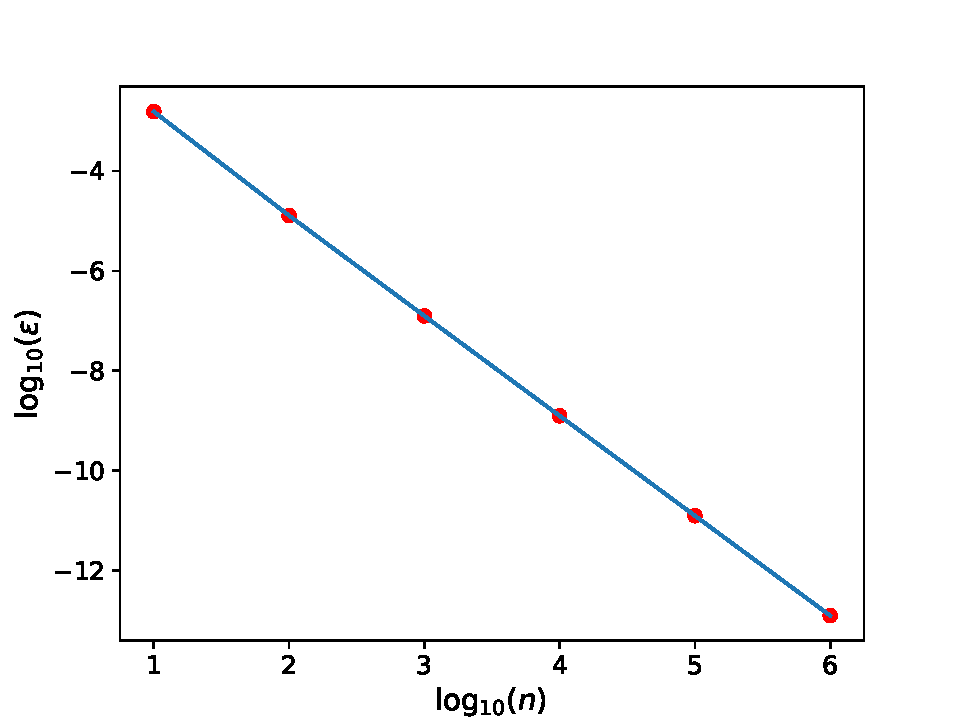
\includegraphics[scale=0.55]{imgs/rel_err.pdf} %Imports the figure.
	\caption{The figure shows the relative error as a function of number of gridpoints $n$ of the estimated integral $\int_0^1 x^3\dd x$ using the midpoint rule.}
	\label{fig:rel_err}
\end{figure}

\textit{Note especially how we reference both the table and the figure with a short explanation of their content. Always do this! In their captions we also typically add additional information such as what we used to produce them. You can also do this in the text if you'd like to. Explain enough so the reader can reproduce them.}

\section{Discussion}
\textit{First note that you are free to merge results and discussions of the results into a single section. This often leads to a more fluid presentation for the reader. On the other hand it's more cumbersome to look at the results a second or third time. Either way, your choice!}

From table \ref{tab:midpoint_rule_tab}, we note that our implementation reproduces the analytical results to a four-digit precision for $n = 10000$ points. This indicates that our implementation is correct.

From figure \ref{fig:rel_err}, the relative error appears to be proportional to $\exp(-\lambda n)$ for some constant $\lambda$, but further investigations of the precise convergence rate of the algorithm should be done.

\textit{Although, a somewhat silly example, you should take note of the following: we are to-the-point with the dicussion and only make strong claims about what we are certain about. We also suggest other avenues of inquiry that was not done in this particular report. Both of these points are important to do. }

\section{Concluding remarks}
\textit{In the "conclusion" section, we state three things in a concise manner: what we did, what the results implied and what should/could be done further.} 

We've looked at an implementation of the midpoint rule. We checked that the implementation indeed reproduced an analytical result which implied its correctly done. Furthermore, we looked at the relative error of the method as a function of number of points. We did not extract a precise convergence rate for the method and suggest this to be a fruitful inquiry for further investigation.
\onecolumngrid
%\bibliographystyle{apalike}
\bibliography{ref}
	
	
\end{document}

